\documentclass{article}
\usepackage{verbatim}
\usepackage{listings}
\usepackage{geometry}
\usepackage{graphicx}
\usepackage{amsmath}
\usepackage{amsthm}
\usepackage{amsfonts}
\usepackage{amssymb}
\geometry{top=2.5cm,bottom=2.5cm,left=2.5cm,right=2.5cm}
\begin{document}
\title{Problem Solving Homework(Week 16)}\author{161180162 Xu Zhiming}\date{\today}
\maketitle
\setlength\parindent{0em}\large\textbf{TC: Chapter 22}\\
\normalsize\textbf{22.1-3}\\
\begin{lstlisting}[language=C,numbers=left]
TRANSPOSE(G)		//Adjacent-list
Build antoher adjacent-list Adj_t//Transposed graph is stored in Adj_t
	for i from 1 to G.V
		for every v in Adj[i]//Original graph is stored in Adj 
			insert v into the front of Adj_t[i]
\end{lstlisting}
Running time:$O(|V|+|E|)$
\begin{lstlisting}[language=C,numbers=left]
TRANSPOSE(G)		//Adjacent-matrix
for i from 1 to G.V //V is the number of vertices in G
	for j from 1 to G.V
		G_t[i][j]=G[j][i]//G_t is the transposed graph
\end{lstlisting}
Running time: $O(|V|^2)$
\textbf{22.1-8}\\
$O(1)$. In this way, we can't easily find the vertices that are adjacent to one vertex, namely, we can only determine whether two vertices are adjacent or not, but can't find a vertex's neighbors.\\ 
\textbf{22.2-3}
\begin{proof}
In the BFS given by the textbook, the three colors: WHITE, GRAY, and BLACK, individually represents a state of a vertex. White for unprocessed, gray for process-needed, black for processed. We can learn from the code that gray isn't of vital importance. Since if we find a white vertex, we just dye it gray and enqueue it. Gray means a intermediate state in order to help us understand. But to the program, this state doesn't have a practical meaning. Because all white vertices are enqueued if discovered. All vertices still in the queue are "gray". Gray is not considered by our code. Therefore, we can remove the color "gray", use only one bit to represent WHITE(unprocessed) and BLACK(processed).
\end{proof}
\textbf{22.2-4}\\
All the vertices are enqueued once, and all their neighbors are explored. Therefore, the algorithm "visits" each vertex twice. The running time is $O(|V|^2)$.\\
\textbf{22.2-5}
\begin{proof}
Suppose now we are exploring vertex $v$'s adjacent-list $Adj[u]$. For every vertex in $Adj[v]$, if they haven't been discovered yet. Their property $d$ is $1+v.d$. So whatever the order in a adjacent-list is, the white vertices among them are always assigned the same $d$.  
\end{proof}
\textbf{22.3-6}
\begin{proof}
\end{proof}
\textbf{22.3-7}
\begin{lstlisting}[language=C,numbers=left]
NONRECURSIVE-DFS(G)
for each vertex u in G.V
	u.color=WHITE
	u.pi=NIL
	time=0
for each vertex u in V
	if u.color==WHITE
	DFS-VISIT(u)
DFS-VISIT(u)
time=time+1
u.d=time
u.color=GRAY
Let s be a new stack
s.push(u)
while s.empty is not true
	u=s.top
	isleaf=true
	for each vertex v in Adj[u]
		if v.color==WHITE
			v.color=GRAY
			v.pi=u
			time=time+1
			v.d=time
			s.push(v)
			isleaf=false
			break
	if isleaf==true
	u.color=BLACK
	time=time+1
	u.f=time
	s.pop
\end{lstlisting}
\textbf{22.2-8}
\begin{figure}[htbp]
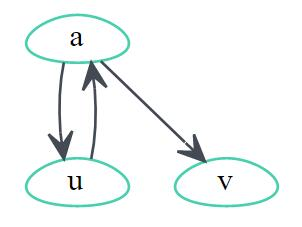
\includegraphics[scale=0.5]{16_1.jpg}
\end{figure}
\\The counterexample are shown above. Explore from $a$.\\
\textbf{22.2-9}
\begin{figure}[htbp]
	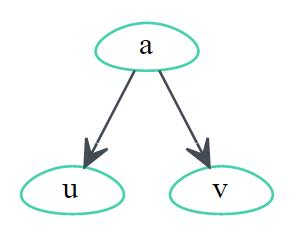
\includegraphics[scale=0.5]{16_2.jpg}
\end{figure}
\\The counterexample are shown above. Explore from $a$. The relation between $v.d$ and $v.f$ is not certain.\\
\textbf{22.2-12}
\begin{lstlisting}[language=C,numbers=left]
DFS-FIND-COMPONETS(G)
for each vertex u in G.V
	u.color=WHITE
	u.pi=NIL
	u.cc=-1
time=0
component=1	//This variant epresses which component a vertex belong to
for each vertex u in G.V
	if u.color==WHITE
		DFS-VISIT(G)
DFS-VISIT(G)
time=time+1
u.d=time
u.cc=component	//"component" is assigned to a vertex's "cc" attribute
for each vertex v in G.Adj[u]
	if v.color==WHITE
		v.pi=u
		v.cc=u.cc
		DFS-VISIT(G)
u.color=BLACK
time=time+1
component=component+1	//This component is done, begin to explore another component
u.f=time
u.color=GRAY	
/*In this way, vertices are in the same component
iff their "cc" attributes are the same*/
\end{lstlisting} 
\textbf{22.4-2}
\begin{lstlisting}[language=C,numbers=left]
NUMBER-OF-PATHS(G)
Let G be an undirected connected graph, s, t are vertices in G
for all v in V
	do v.num_p<-0
TOPOLOGICAL-SORT(G)
	s.num_p<-1
for each v in V in topologically sorted order
	do if v.num>s.sum
		for each u in Adj[v]
			u.num_p=u.num_p+v.num_p
return u.num_p		 
\end{lstlisting}
\textbf{22.4-3}
\begin{lstlisting}[language=C,numbers=left]
GRAPH-CYCLE(G)
if DFS(G) doesn't yield back egdes
	an undirected graph is acycle.
if there is a back egde
	return the graph contains a cycle
if there is no back edge
	return the graph is acycle
\end{lstlisting}
\textbf{22.5-5}
\begin{lstlisting}[language=C,numbers=left]
STRONG-CONNECTED-COMPONENTS(G)
Consider the vertices in the form of strong connected components, choose a vertex in each components into G_SCC
Traverse the edge in G(V,E) and add edge in G_SCC correspondingly. 
\end{lstlisting}
Total cost: $\Theta(|V|+|E|)$\\
\textbf{22.5-7}
\begin{lstlisting}[language=C,numbers=left]
STRONG-CONNECTED-COMPONENTS(G)
COMPONENT(G)
TOPOLOGOICALLY(G)
verify that the sequence of vertices (v[1],v[2],...,v[k]) given by topological sort.
If the vertices form a linear chain
	the original graph is semiconnected
else
	it is not
\end{lstlisting}
Running time: $\Theta(|V|+|E|)$
\end{document}

